% -*- TeX -*- -*- UK -*-
% ----------------------------------------------------------------
% arXiv Paper ************************************************
%
% Subhaneil Lahiri's template
%
% Before submitting:
%    Comment out hyperref
%    Comment out showkeys
%    Replace \newcommand{\mlim}[2]{{\stackrel{\scriptstyle #1}{#2}}}
\newcommand{\ra}{\rightarrow}
\newcommand{\lr}{\leftrightarrow}
\newcommand{\cdt}{\!\cdot\!}
\newcommand{\vp}{\vspace{0.5cm}}
\newcommand{\degs}{^\circ}
%
%e.g., i.e. with normal spaces
\newcommand{\eg}{e.g.\ }
\newcommand{\ie}{i.e.\ }
\newcommand{\cf}{cf.\ }
\newcommand{\etc}{etc.\ }
%
% indices
\newcommand{\up}[1]{\mbox{}^{#1}}
\newcommand{\dn}[1]{\mbox{}_{#1}}
\newcommand{\rp}[1]{^{(#1)}}
\newcommand{\lp}[1]{_{(#1)}}
%
% brackets etc.
\newcommand{\prn}[1]{\left ( #1 \right )}
\newcommand{\brc}[1]{\left\{ #1 \right\}}
\newcommand{\brk}[1]{\left [ #1 \right ]}
\newcommand{\abs}[1]{\left\lvert #1 \right\rvert}
\newcommand{\nrm}[1]{\left\lVert #1 \right\rVert}
\newcommand{\av}[1]{\left\langle #1 \right\rangle}
%
% QM Dirac notation
\newcommand{\bra}[1]{\left\langle #1 \right \rvert}
\newcommand{\ket}[1]{\left \lvert #1 \right\rangle}
\newcommand{\braket}[2]{\left\langle #1 \midddle | #2 \right\rangle}
\newcommand{\bracket}[3]{\left\langle #1 \middle | #2 \middle | #3 \right\rangle}
%
% Derivatives, etc. First argument is optional.
\newcommand{\diff}[3][\rule{0mm}{0mm}]{\frac{\mathrm{d}^{#1} #2}{\mathrm{d}{#3}^{#1}}}
\newcommand{\pdiff}[3][\rule{0mm}{0mm}]{\frac{\partial^{#1} #2}{\partial {#3}^{#1}}}
\newcommand{\pdiffc}[3][\rule{0mm}{0mm}]{\left (\frac{\partial #2}{\partial {#3}}\right )_{\!\!#1}}
\newcommand{\pdl}[1][\rule{0mm}{0mm}]{\overleftarrow{\partial}_{#1}}
\newcommand{\pdr}[1][\rule{0mm}{0mm}]{\overrightarrow{\partial}_{#1}}
\newcommand{\pdlr}[1][\rule{0mm}{0mm}]{\overleftrightarrow{\partial_{#1}}}
\newcommand{\fdf}[2]{\frac{\delta #1}{\delta #2}}
\newcommand{\intd}[1]{\int\!\dr #1\,}
%
% Un-italicised letters
\newcommand{\dr}{\mathrm{d}}
\newcommand{\e}{\mathrm{e}}
\newcommand{\ir}{\mathrm{i}}
\DeclareMathOperator{\tr}{tr}
\DeclareMathOperator{\Tr}{Tr}
\DeclareMathOperator{\Det}{Det}
%
% The default \Im and \Re look crap
\renewcommand{\Im}{\operatorname{\mathfrak{Im}}}
\renewcommand{\Re}{\operatorname{\mathfrak{Re}}}
%
% Referencing sections, figures, etc
\newcommand{\sref}[1]{\S\ref{#1}}
\newcommand{\cref}[1]{Ch.\ref{#1}}
\newcommand{\Cref}[1]{Ch.\ref{#1}}
\newcommand{\fref}[1]{fig.\ref{#1}}
\newcommand{\Fref}[1]{Fig.\ref{#1}}
\newcommand{\tref}[1]{tab.\ref{#1}}
\newcommand{\Tref}[1]{Tab.\ref{#1}}
%
\newcommand{\nn}{\nonumber}
%
% Put the preprint numbers in the top right corner of the page.
% Use after \maketitle.
% First argument: How high it needs to be raised,
% Second argument: Width of the box,
% Third argument: The preprint numbers.
\newcommand{\preprintno}[3]{\hfill\raisebox{#1}[0cm][0cm]{
\begin{minipage}[t]{#2}\begin{flushright} #3 \end{flushright}\end{minipage}}
\vspace*{-\baselinestretch\baselineskip}}
%
% If you have changed the line spacing, e.g. with \renewcommand{\baselinestretch}{1.5},
% the command \sgap produces a line break with the normal spacing.
\newlength{\lingap}
\setlength{\lingap}{\baselinestretch\baselineskip}
\addtolength{\lingap}{-\baselineskip}
\newcommand{\sgap}{\\[-\lingap]}
 with its contents
%       or include mydefs.tex in zip/tar file
%    Replace %
\newcommand{\CD}{\mathcal{D}}
\newcommand{\CE}{\mathcal{E}}
\newcommand{\CG}{\mathcal{G}}
\newcommand{\CH}{\mathcal{H}}
\newcommand{\CK}{\mathcal{K}}
\newcommand{\CO}{\mathcal{O}}
\newcommand{\CL}{\mathcal{L}}
\newcommand{\CM}{\mathcal{M}}
\newcommand{\CN}{\mathcal{N}}
\newcommand{\CV}{\mathcal{V}}
\newcommand{\CZ}{\mathcal{Z}}
%
\newcommand{\dM}{\mathfrak{M}}
\newcommand{\dmd}{\mathfrak{d}}
\newcommand{\dmD}{\mathfrak{D}}
%
\newcommand{\R}{\mathbb{R}}
\newcommand{\C}{\mathbb{C}}
\newcommand{\CP}{\mathbb{CP}}
\newcommand{\Z}{\mathbb{Z}}
%
\newcommand{\ad}{{\dot{\alpha}}}
\newcommand{\bd}{{\dot{\beta}}}
\newcommand{\gd}{{\dot{\gamma}}}
\newcommand{\dd}{{\dot{\delta}}}
\newcommand{\ed}{{\dot{\epsilon}}}
%
\newcommand{\bs}{\overline{\sigma}}
\newcommand{\br}{\overline{\rho}}
\newcommand{\bpsi}{\overline{\psi}}
\newcommand{\bchi}{\overline{\chi}}
\newcommand{\bPsi}{\overline{\Psi}}
\newcommand{\bQ}{\overline{Q}}
\newcommand{\bS}{\overline{S}}
\newcommand{\bJ}{\overline{J}}
\newcommand{\zb}{{\bar z}}
\newcommand{\wb}{{\overline w}}
\newcommand{\cb}{{\bar c}}
\newcommand{\ab}{{\bar a}}
\newcommand{\bb}{{\bar b}}
\newcommand{\bp}{{\bar\partial}}
%
\newcommand{\p}{\partial}
\newcommand{\apm}{{\alpha^{\prime}}}
\newcommand{\adg}{a^\dagger}
\newcommand{\psq}{^{\prime\,2}}
\newcommand{\ppsq}{^{\prime\prime\,2}}
\newcommand{\half}{\frac{1}{2}}
%
 with its contents
%       or include newsymb.tex in zip/tar file
%    Put this file, the .bbl file, any picture or
%       other additional files and natbib.sty
%       file in a zip/tar file
%
% **** -----------------------------------------------------------
\documentclass[12pt]{article}
% Preamble:
\usepackage{a4wide}
\usepackage[centertags]{amsmath}
\usepackage{amssymb}
%\usepackage{amsthm}
\usepackage[sort&compress,numbers]{natbib}
%\usepackage{citeB}
\usepackage{ifpdf}
\usepackage{graphicx}
%\usepackage{graphics} for finding documentation only
%\usepackage{xcolor}
%\usepackage{pgf}
\ifpdf
\usepackage[pdftex,bookmarks]{hyperref}
\else
\usepackage[hypertex]{hyperref}
\DeclareGraphicsRule{.png}{eps}{.bb}{}
\fi
\usepackage{epstopdf}
\epstopdfsetup{update,suffix=-generated}
%
% >> Only for drafts! <<
\usepackage[notref,notcite]{showkeys}
% ----------------------------------------------------------------
\vfuzz2pt % Don't report over-full v-boxes if over-edge is small
\hfuzz2pt % Don't report over-full h-boxes if over-edge is small
%\numberwithin{equation}{section}
%\renewcommand{\baselinestretch}{1.5}
% ----------------------------------------------------------------
% New commands etc.
\newcommand{\mlim}[2]{{\stackrel{\scriptstyle #1}{#2}}}
\newcommand{\ra}{\rightarrow}
\newcommand{\lr}{\leftrightarrow}
\newcommand{\cdt}{\!\cdot\!}
\newcommand{\vp}{\vspace{0.5cm}}
\newcommand{\degs}{^\circ}
%
%e.g., i.e. with normal spaces
\newcommand{\eg}{e.g.\ }
\newcommand{\ie}{i.e.\ }
\newcommand{\cf}{cf.\ }
\newcommand{\etc}{etc.\ }
%
% indices
\newcommand{\up}[1]{\mbox{}^{#1}}
\newcommand{\dn}[1]{\mbox{}_{#1}}
\newcommand{\rp}[1]{^{(#1)}}
\newcommand{\lp}[1]{_{(#1)}}
%
% brackets etc.
\newcommand{\prn}[1]{\left ( #1 \right )}
\newcommand{\brc}[1]{\left\{ #1 \right\}}
\newcommand{\brk}[1]{\left [ #1 \right ]}
\newcommand{\abs}[1]{\left\lvert #1 \right\rvert}
\newcommand{\nrm}[1]{\left\lVert #1 \right\rVert}
\newcommand{\av}[1]{\left\langle #1 \right\rangle}
%
% QM Dirac notation
\newcommand{\bra}[1]{\left\langle #1 \right \rvert}
\newcommand{\ket}[1]{\left \lvert #1 \right\rangle}
\newcommand{\braket}[2]{\left\langle #1 \midddle | #2 \right\rangle}
\newcommand{\bracket}[3]{\left\langle #1 \middle | #2 \middle | #3 \right\rangle}
%
% Derivatives, etc. First argument is optional.
\newcommand{\diff}[3][\rule{0mm}{0mm}]{\frac{\mathrm{d}^{#1} #2}{\mathrm{d}{#3}^{#1}}}
\newcommand{\pdiff}[3][\rule{0mm}{0mm}]{\frac{\partial^{#1} #2}{\partial {#3}^{#1}}}
\newcommand{\pdiffc}[3][\rule{0mm}{0mm}]{\left (\frac{\partial #2}{\partial {#3}}\right )_{\!\!#1}}
\newcommand{\pdl}[1][\rule{0mm}{0mm}]{\overleftarrow{\partial}_{#1}}
\newcommand{\pdr}[1][\rule{0mm}{0mm}]{\overrightarrow{\partial}_{#1}}
\newcommand{\pdlr}[1][\rule{0mm}{0mm}]{\overleftrightarrow{\partial_{#1}}}
\newcommand{\fdf}[2]{\frac{\delta #1}{\delta #2}}
\newcommand{\intd}[1]{\int\!\dr #1\,}
%
% Un-italicised letters
\newcommand{\dr}{\mathrm{d}}
\newcommand{\e}{\mathrm{e}}
\newcommand{\ir}{\mathrm{i}}
\DeclareMathOperator{\tr}{tr}
\DeclareMathOperator{\Tr}{Tr}
\DeclareMathOperator{\Det}{Det}
%
% The default \Im and \Re look crap
\renewcommand{\Im}{\operatorname{\mathfrak{Im}}}
\renewcommand{\Re}{\operatorname{\mathfrak{Re}}}
%
% Referencing sections, figures, etc
\newcommand{\sref}[1]{\S\ref{#1}}
\newcommand{\cref}[1]{Ch.\ref{#1}}
\newcommand{\Cref}[1]{Ch.\ref{#1}}
\newcommand{\fref}[1]{fig.\ref{#1}}
\newcommand{\Fref}[1]{Fig.\ref{#1}}
\newcommand{\tref}[1]{tab.\ref{#1}}
\newcommand{\Tref}[1]{Tab.\ref{#1}}
%
\newcommand{\nn}{\nonumber}
%
% Put the preprint numbers in the top right corner of the page.
% Use after \maketitle.
% First argument: How high it needs to be raised,
% Second argument: Width of the box,
% Third argument: The preprint numbers.
\newcommand{\preprintno}[3]{\hfill\raisebox{#1}[0cm][0cm]{
\begin{minipage}[t]{#2}\begin{flushright} #3 \end{flushright}\end{minipage}}
\vspace*{-\baselinestretch\baselineskip}}
%
% If you have changed the line spacing, e.g. with \renewcommand{\baselinestretch}{1.5},
% the command \sgap produces a line break with the normal spacing.
\newlength{\lingap}
\setlength{\lingap}{\baselinestretch\baselineskip}
\addtolength{\lingap}{-\baselineskip}
\newcommand{\sgap}{\\[-\lingap]}

%
\newcommand{\CD}{\mathcal{D}}
\newcommand{\CE}{\mathcal{E}}
\newcommand{\CG}{\mathcal{G}}
\newcommand{\CH}{\mathcal{H}}
\newcommand{\CK}{\mathcal{K}}
\newcommand{\CO}{\mathcal{O}}
\newcommand{\CL}{\mathcal{L}}
\newcommand{\CM}{\mathcal{M}}
\newcommand{\CN}{\mathcal{N}}
\newcommand{\CV}{\mathcal{V}}
\newcommand{\CZ}{\mathcal{Z}}
%
\newcommand{\dM}{\mathfrak{M}}
\newcommand{\dmd}{\mathfrak{d}}
\newcommand{\dmD}{\mathfrak{D}}
%
\newcommand{\R}{\mathbb{R}}
\newcommand{\C}{\mathbb{C}}
\newcommand{\CP}{\mathbb{CP}}
\newcommand{\Z}{\mathbb{Z}}
%
\newcommand{\ad}{{\dot{\alpha}}}
\newcommand{\bd}{{\dot{\beta}}}
\newcommand{\gd}{{\dot{\gamma}}}
\newcommand{\dd}{{\dot{\delta}}}
\newcommand{\ed}{{\dot{\epsilon}}}
%
\newcommand{\bs}{\overline{\sigma}}
\newcommand{\br}{\overline{\rho}}
\newcommand{\bpsi}{\overline{\psi}}
\newcommand{\bchi}{\overline{\chi}}
\newcommand{\bPsi}{\overline{\Psi}}
\newcommand{\bQ}{\overline{Q}}
\newcommand{\bS}{\overline{S}}
\newcommand{\bJ}{\overline{J}}
\newcommand{\zb}{{\bar z}}
\newcommand{\wb}{{\overline w}}
\newcommand{\cb}{{\bar c}}
\newcommand{\ab}{{\bar a}}
\newcommand{\bb}{{\bar b}}
\newcommand{\bp}{{\bar\partial}}
%
\newcommand{\p}{\partial}
\newcommand{\apm}{{\alpha^{\prime}}}
\newcommand{\adg}{a^\dagger}
\newcommand{\psq}{^{\prime\,2}}
\newcommand{\ppsq}{^{\prime\prime\,2}}
\newcommand{\half}{\frac{1}{2}}
%

%
%%%%%%%%%%%%%%%%%%%%%%%%%%%%%%%%%%%%%%%%%%%%%%%%%%%%%%%%%%%%%%%%%%%%%%%%%%
% Title info:
\title{Mutual information between successive reorientations}
%
% Author List:
%
\author{Subhaneil Lahiri
\\
%
% Addresses:
%
\small{\emph{Harvard University,}}
%
}

\begin{document}

\maketitle



%%%%%%%%%%%%%%%%%%%%%%%%%%%%%%%%%%%%%%%%%%%%%%%%%%%%%%%%%%%%%%%%%%%%%%%%%%


\begin{abstract}
  We show how mutual information can be used to describe the independence of successive reorientations
\end{abstract}


%%%%%%%%%%%%%%%%%%%%%%%%%%%%%%%%%%%%%%%%%%%%%%%%%%%%%%%%%%%%%%%%%%%%%%%%%%
% Beginning of Article:
%%%%%%%%%%%%%%%%%%%%%%%%%%%%%%%%%%%%%%%%%%%%%%%%%%%%%%%%%%%%%%%%%%%%%%%%%%

\section{Reorientation sequences}\label{sec:reoseq}

As a worm navigates, it performs a sequence of turns. When turns occur sufficiently close to each other, they are grouped into a reorientation event. These reorientations have several characteristics, \eg the types of turn of which it is composed, the difference in heading direction before and after, the duration of the run leading into it. We wish to know if the characteristics of one reorientation are independent of the characteristics of previous reorientations.

Consider a sequence of $r$ successive reorientations. The values of a particular characteristic of these reorientations is an $r$-tuple of random variables: $(X_1,\ldots,X_r)$. We are asking whether or not $P(X_1,\ldots,X_r) = P(X_1)\ldots P(X_r)$. We will discuss some measures of independence in \sref{sec:entropy}.

These probability distributions can be estimated from the frequencies in a sample sequence (described schematically in \fref{fig:schematic}). However, as a consequence of finite sample size, this process has both systematic and random errors. We will look at several methods for removing systematic errors in \sref{sec:syscorr} and one method for estimating random errors in appendix \ref{sec:stderr}.

In principle we should look at all the characteristics together. However, increasing the dimensionality of the data at each reorientation increases the number of bins used, which in turn increases the number of samples needed. Therefore, we will have to be satisfied with looking at each characteristic separately.

\begin{figure}
  \begin{center}
    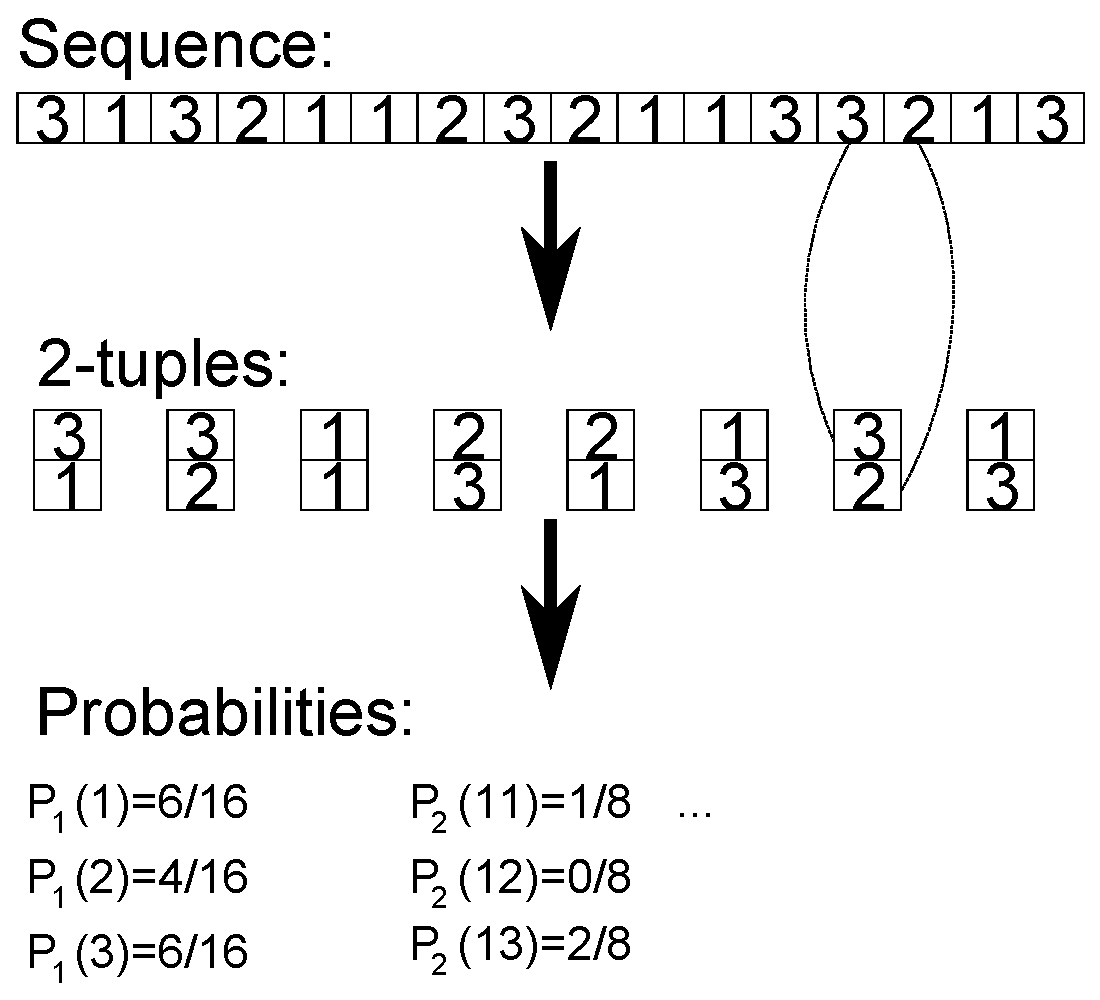
\includegraphics[width=10cm]{schematic.eps}
  \end{center}
  %\input{.TpX}
  \caption{Schematic calculation of probabilities. (a) Sample sequence of reorientations. (b) Grouping sequence into $r$-tuples ($r=2$). (c) Estimating probabilities for individual members and for $r$-tuples from relative frequencies in sample.} \label{fig:schematic}
\end{figure}



\section{Entropy and mutual information}\label{sec:entropy}

The \textbf{entropy} of a probability distribution is a measure of the lack of information we have about a random variable:
%
\begin{equation}\label{eq:ent}
  H(X) = \av{-\log P(X)}.
\end{equation}
%
It takes its minimum value of $0$ when $X$ can only take one value. It takes its maximum value of $\log n$ when $X$ has a uniform distribution over $n$ possibilities.

With several random variables, we can define a joint entropy from their joint probability distribution:
%
\begin{equation}\label{eq:jointent}
  H(X_1,\ldots,X_r) = \av{-\log P(X_1,\ldots,X_r)}.
\end{equation}
%
It satisfies the bounds
%
\begin{equation}\label{eq:entbounds}
  \max_i H(X_i) \leq H(X_1,\ldots,X_r) \leq \sum_{i=1}^r H(X_i).
\end{equation}
%
The lower bound is saturated when one of the variables is enough to determine the others. The upper bound is saturated when the $X_i$ are independent:
%
\begin{equation}\label{eq:indent}
  P(X1,\ldots,X_r) = \prod_{i=1}^r P(X_i)
  \quad \implies \quad
  H(X_1,\ldots,X_r) = \sum_{i=1}^r H(X_i).
\end{equation}
%

We can define the following measure of (lack of) independence:
%
\begin{equation}\label{eq:mutinf}
  I(X_1,\ldots,X_r) = \sum_{i=1}^r H(X_i) - H(X_1,\ldots,X_r).
\end{equation}
%
In the case $r=2$, this is the \textbf{mutual information} between $X_1$ and $X_2$. For $r>2$, there are many different generalisations of mutual information. This one is called the \textbf{total correlation} \cite{Watanabe:1960:ITA:1661258.1661265}, or multiinformation. It has the properties:
%
\begin{itemize}
  \item it vanishes if and only if the random variables are independent
  \item otherwise, it is positive.
  \item it is bounded from above by $\sum_{i=1}^r H(X_i) - \max_i H(X_i)$.
\end{itemize}
%

In our cases, the random variables, $X_i$, all have the same distribution, so the total correlation satisfies the bounds
%
\begin{equation}\label{eq:mutinfbounds}
  0 \leq I_r(X_1,\ldots,X_r) \leq (r-1)H(X).
\end{equation}
%
We can define a normalised total correlation:
%
\begin{equation}\label{eq:normmutinf}
  C_r = \frac{I_r}{(r-1)H_1}, \qquad 0 \leq C_r \leq 1.
\end{equation}
%
The lower bound corresponds to complete independence. The upper bound corresponds to complete redundancy.


\section{Correcting systematic errors}\label{sec:syscorr}

We will compute the quantities defined in the previous section by estimating the probability distributions, $P_1(X_i)$ and $P_r(X_1,\ldots,X_r)$ from the relative frequencies in sample sequences of reorientations. As all the $X_i$ have the same distribution, we will estimate $P_1(X)$ from the pooled data, rather that estimating the $P_1(X_i)$ separately. When looking at reorientation types, we will restrict attention to the 5 most common types. When looking at angles and run durations, the data has to be binned. We will follow the approach of \cite{2005cs........2017S} and place the bins on quantiles of the data, preserving the coordinate invariance of the mutual information. In both cases, we will use 5 bins.


The lower bounds on mutual information, \eqref{eq:mutinfbounds} and \eqref{eq:normmutinf}, lead to systematic errors which tend to bias these estimates upwards. There are several methods for estimating this bias.

One approach involves expending the errors in one over the sample size, see \cite{1999PhyD..125..285R} and estimating the leading order correction. One can also estimate the random errors using this approach. Our estimators are slightly different to those used there, the appropriate versions of the estimates are calculated in Appendix \ref{sec:stderr}.

As the bias estimates are independent of the actual probability distribution, depending only on sample size and number of bins, we can estimate the bias by computing the mutual information for a completely random sequence in the same way. As the true value is zero, the result of this computation is an estimate of the bias. Furthermore, if the probabilities of the individual elements of the sequence are the same as in the data, this can be regarded as a Monte-Carlo simulation of the null hypothesis -- that the individual elements of the sequence are independent of each other. Thus, we can compute a p-value by seeing where the original result ranks amongst the results of the simulation.

We will do this using the non-parametric bootstrap. This is conceptually similar to the common alternative procedure of shuffling the sequence. Shuffling can be thought of as resampling without replacement, whereas the non-parametric bootstrap is resampling with replacement. They both involve removing any information in the sequence without changing the probabilities of the individual elements.

The direct method of \cite{1998PhRvL..80..197S} consists of varying the sample size and extrapolating to infinity. This can also be used to check that the number of samples is large enough compared to the number of bins. With this method, it is difficult to compute error bars and p-values, as the process is slow.

We show three examples of these methods in \fref{fig:biascomp}, one where they agreed really well, one where the agreement was not too bad and one where it was terrible, probably indicating that the sample size is too small.


\begin{figure}
  \begin{center}
    (a)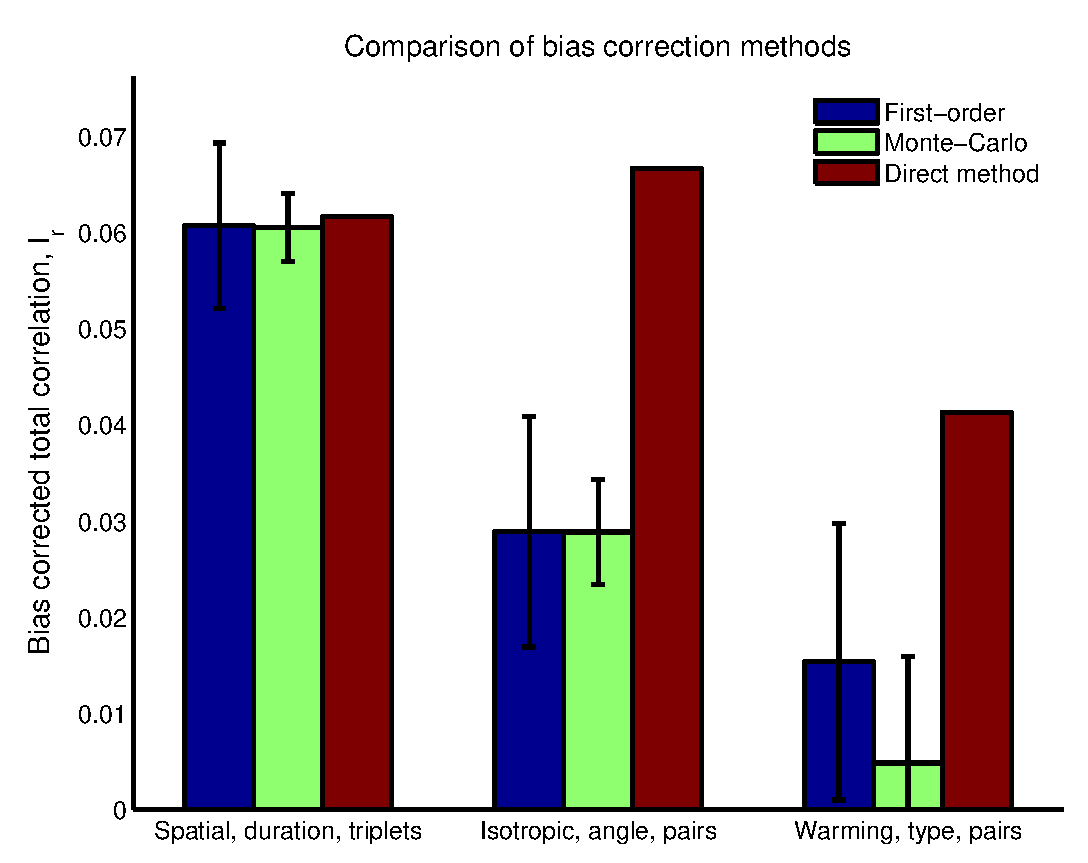
\includegraphics[width=7cm]{comparison.eps}
    (b)i)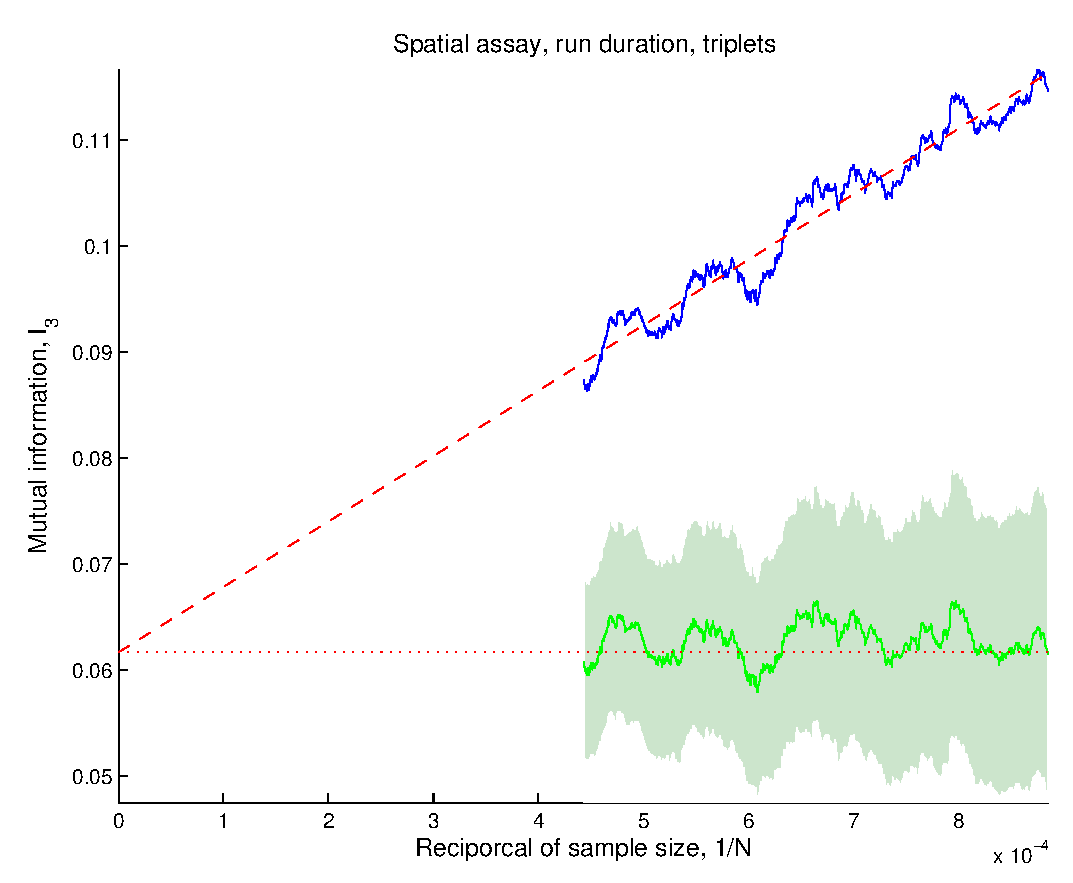
\includegraphics[width=7cm]{spat_dur_3.eps}\\
    ii)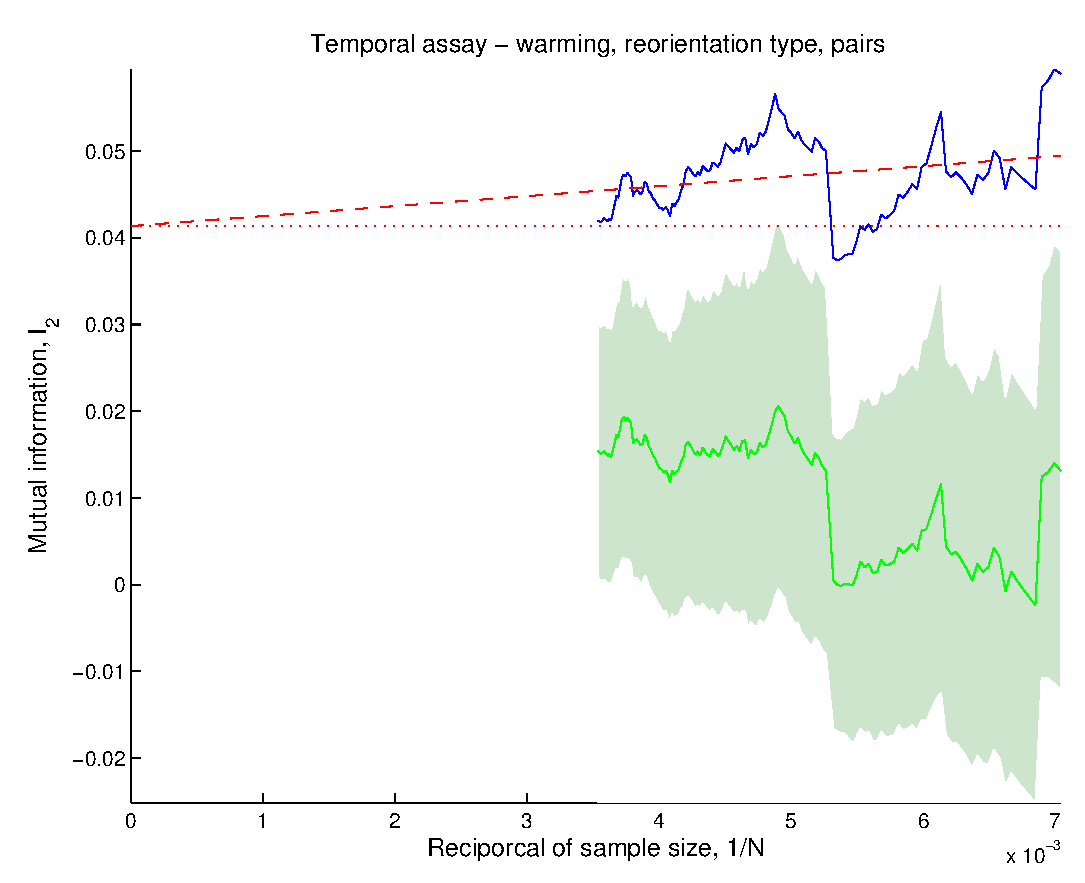
\includegraphics[width=7cm]{warm_typ_2.eps}
    iii)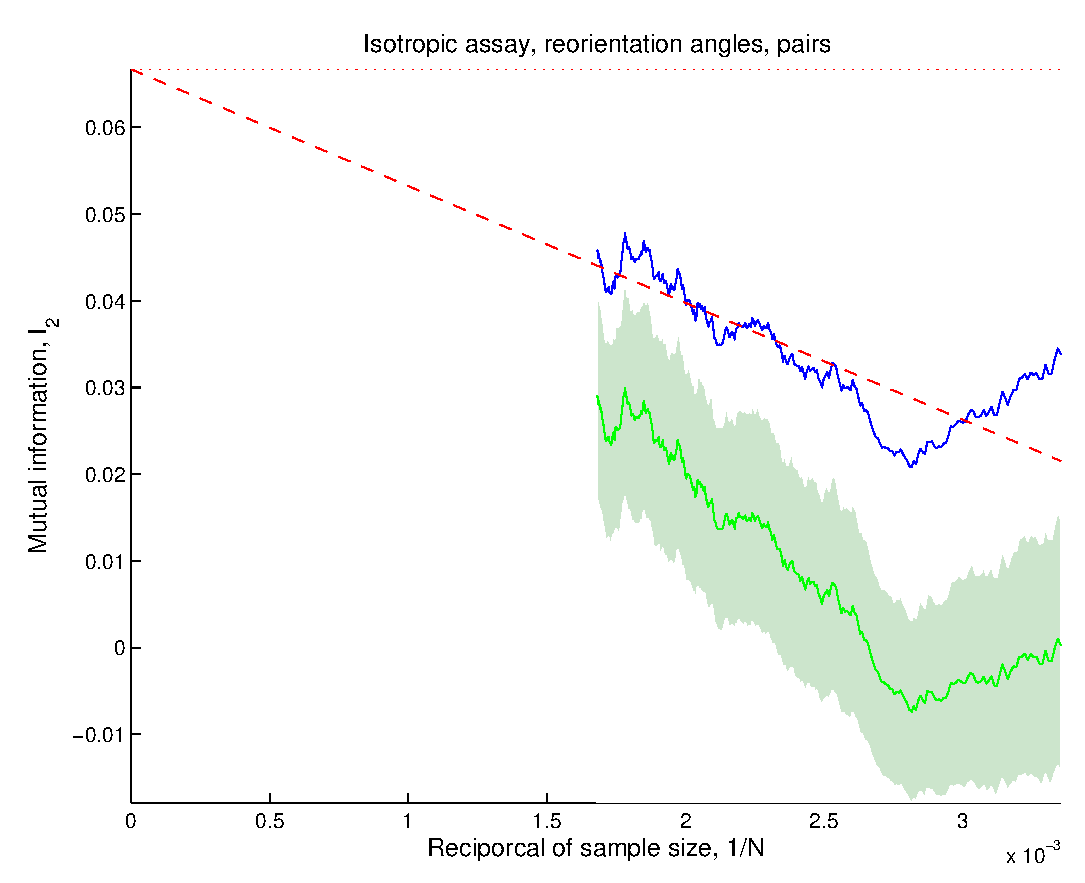
\includegraphics[width=7cm]{iso_ang_2.eps}
  \end{center}
  \caption{Comparison of different methods for removing bias. (a) Three examples of the three unbiased estimates of mutual information/total correlation. First-order refers to the methods of appendix \ref{sec:stderr}. Monte-Carlo refers to subtracting the mean of 1000 nonparametric bootstrap simulations, the error-bars are the standard deviation of the bootstrap simulations. (b) Illustration of the direct method, Blue line is the uncorrected estimates with different sample sizes, red dashed line shows the extrapolation to infinite sample size and red dotted line indicates the result of this extrapolation. Green line shows the unbiased estimator using the first-order method of appendix \ref{sec:stderr} for comparison, darker green shading is $\pm$ one standard error. i)-iii) the three cases shown in (a).} \label{fig:biascomp}
\end{figure}

\section{Results}\label{sec:results}

\begin{figure}
  \begin{center}
    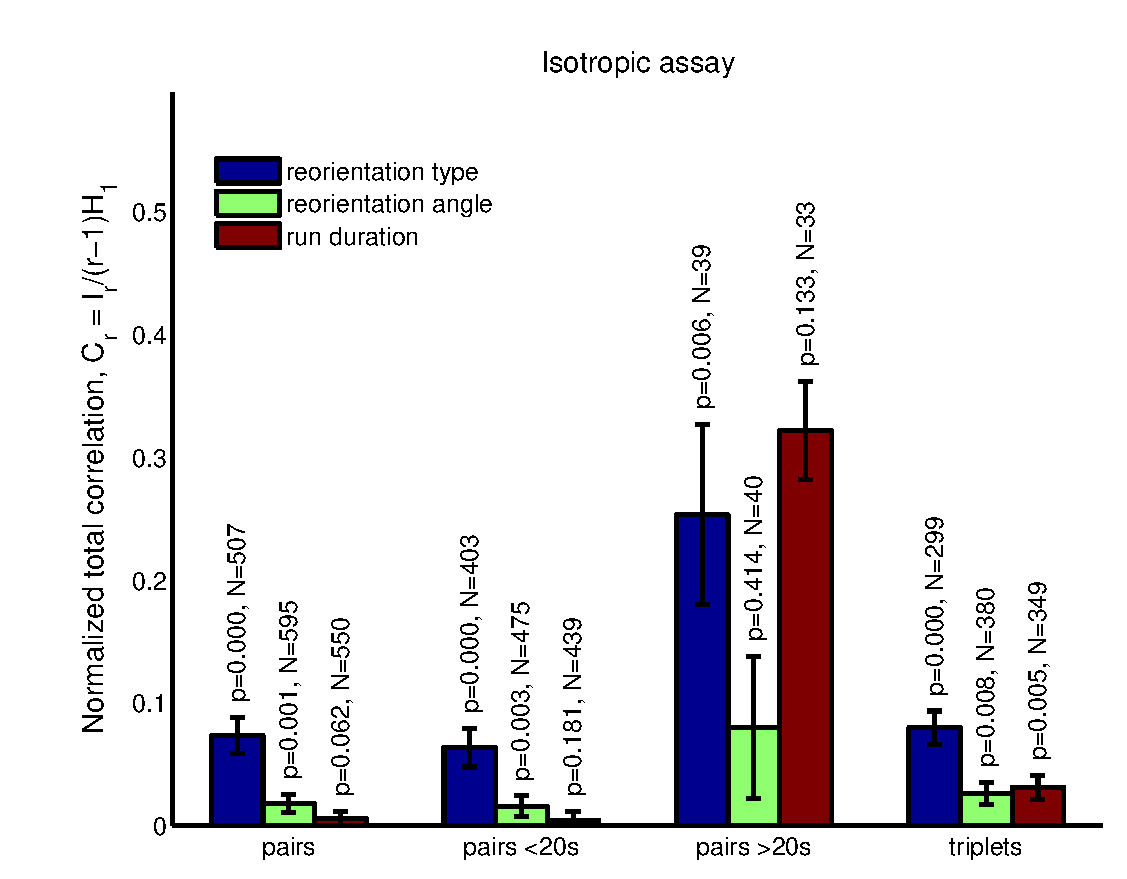
\includegraphics[width=8cm]{isotropic.eps}
    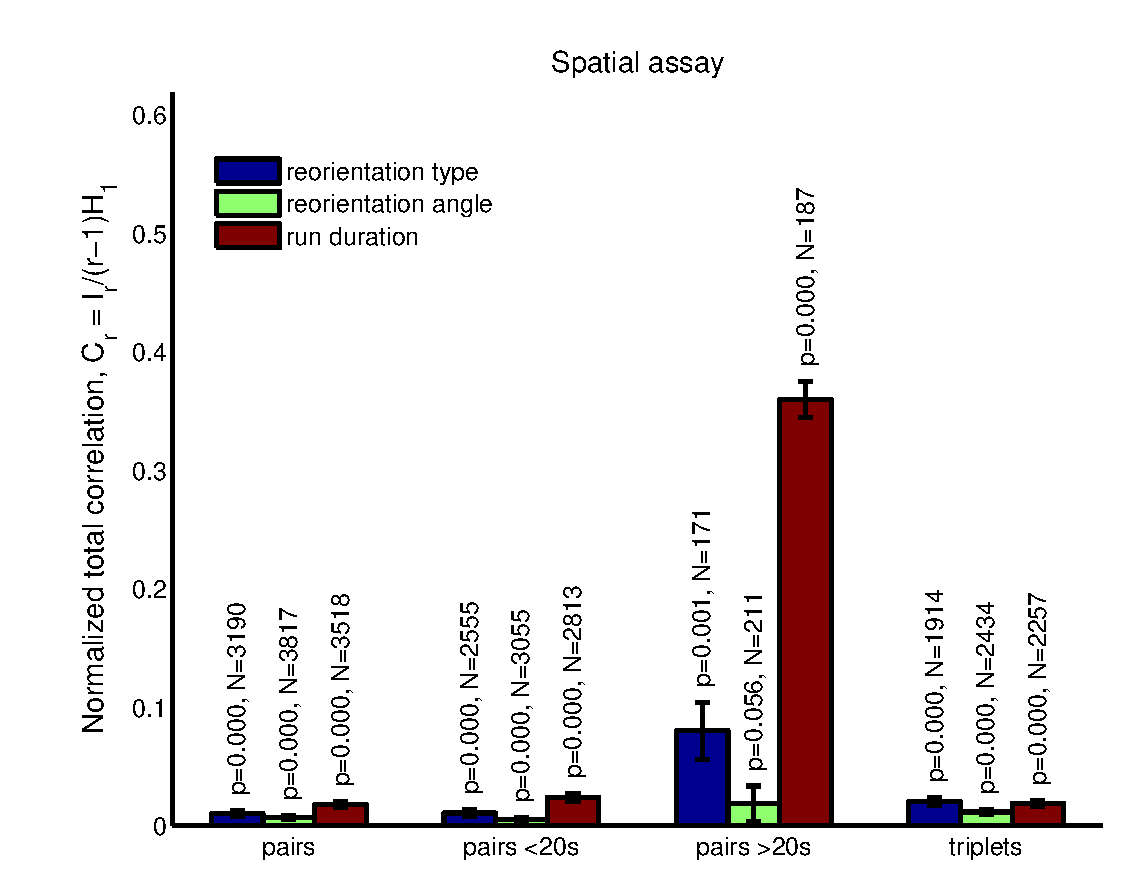
\includegraphics[width=8cm]{spatial.eps}\\
    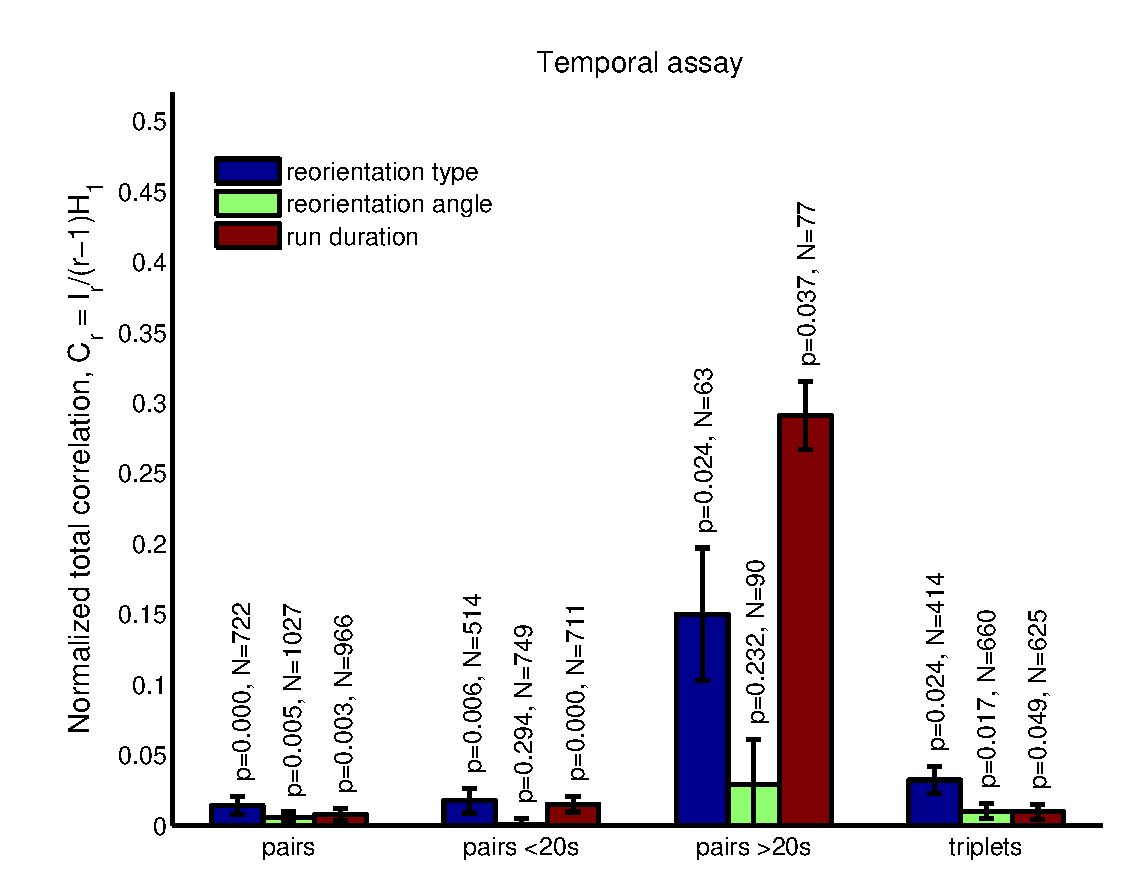
\includegraphics[width=8cm]{temporal.eps}
    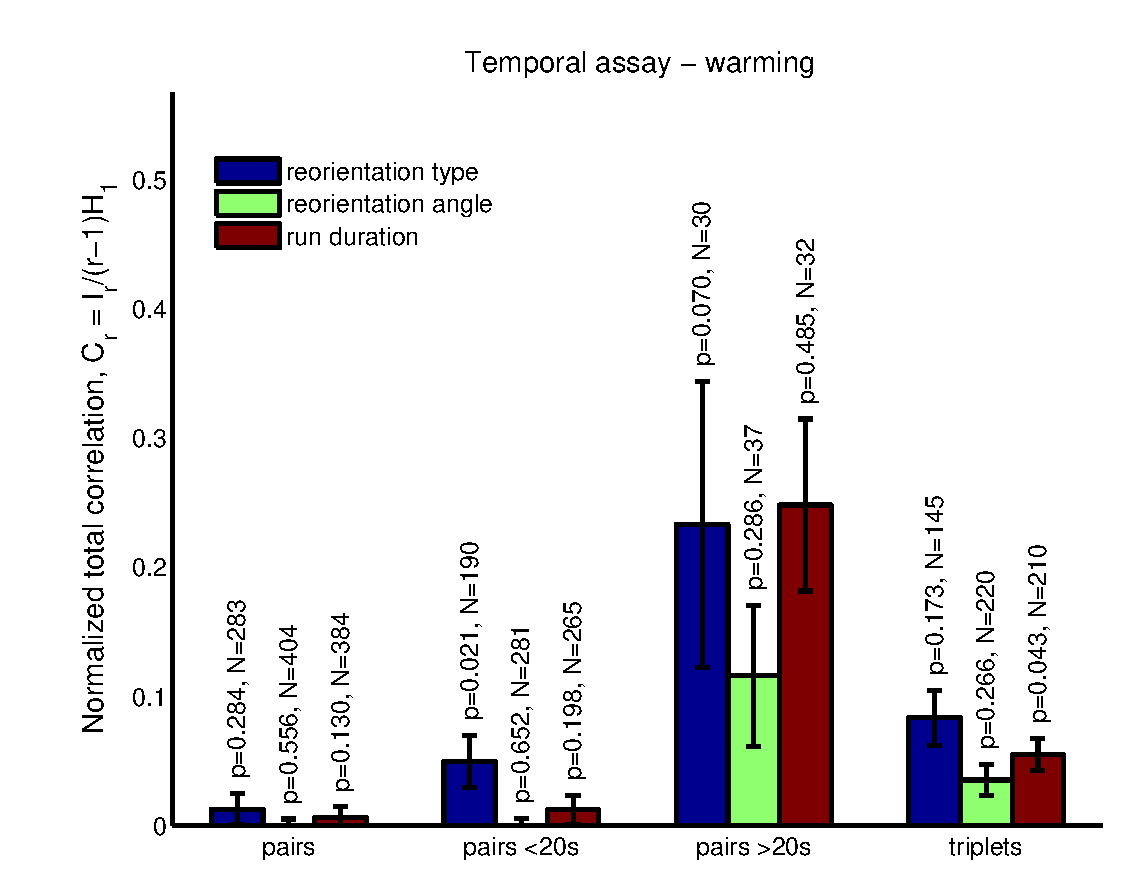
\includegraphics[width=8cm]{warming.eps}\\
    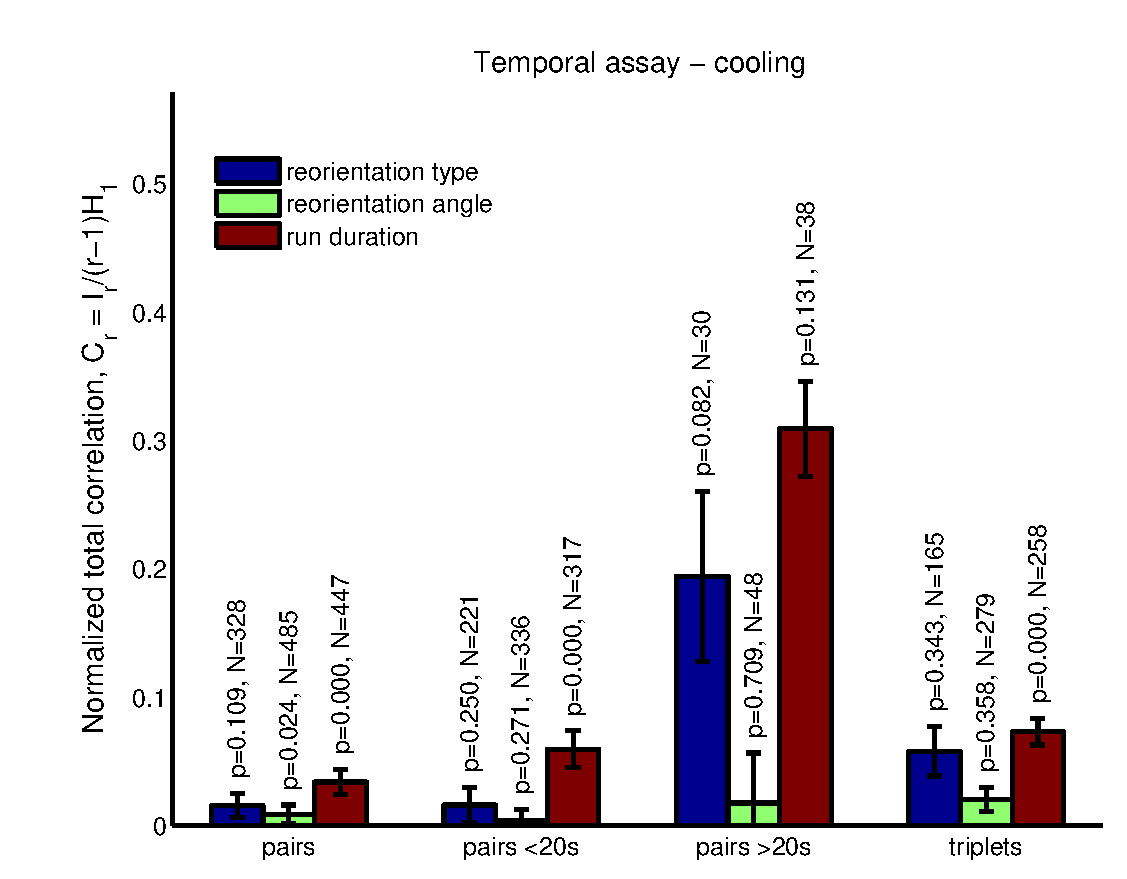
\includegraphics[width=8cm]{cooling.eps}
  \end{center}
  \caption{Normalised total correlation/mutual information}\label{fig:results}
\end{figure}


\appendix\section*{Appendices}

\section{Bias and standard error}\label{sec:stderr}

We will follow the approach of \cite{1999PhyD..125..285R}. Our situation is slightly different from that one. As all the $X_i$ have the same distribution, we will estimate $P(X)$ from the pooled data, rather that estimating the $P(X_i)$ separately. This means that our estimates may not satisfy the bounds, such as \eqref{eq:mutinfbounds}.

Let $p_{i_1\ldots i_r}$ denote the probability $P_r(X_1=x_{i_1},\ldots,X_r=x_{i_r})$ and $n_{i_1\ldots i_r}$ denote the number of corresponding r-tuples in the sample. We can estimate $p_{i_1\ldots i_r}$ with
%
\begin{equation}\label{eq:tupprob}
  q_{i_1\ldots i_r} = \frac{n_{i_1\ldots i_r}}{N},
  \qquad
  N = \sum_{j_1\ldots ji_r} n_{j_1\ldots j_r}.
\end{equation}
%
We can then estimate $p_{j}=P_1(X=x_{j})$ with
%
\begin{equation}\label{eq:singprob}
  q_j = \sum_{i_1\ldots i_r}\prn{ \frac{q_{i_1\ldots i_r}}{r} \sum_{a=1}^r \delta_{j,i_a}}.
\end{equation}
%

From now on, we will use $A$ to denote the estimate of $A(p)$ with $p$ replaced by $q$ and $\widehat{A}=A-\bias(A)$, where $A$ is one of $(H_1,H_r,I_r,C_r)$.

Our bias estimates are essentially the same as those of \cite{1999PhyD..125..285R}, except that the number of samples for $H_1$ is $rN$ rather than $N$:
%
\begin{equation}\label{eq:biasH}
  B_1 = \bias(H_1) = -\frac{\#b_1}{2rN},
  \qquad
  B_r = \bias(H_r) = -\frac{\#b_r}{2N},
\end{equation}
%
where $\#b_r$ is the number of non-empty bins (\eg in \fref{fig:schematic}, $\#b_1=3$, $\#b_2=6$). The bias estimate for $I$ and $C$ follow in the usual way.

We can estimate the standard errors with
%
\begin{equation}\label{eq:stderr}
  \var(A) \approx \sum_{i_1\ldots i_r} \prn{\pdiff{A}{n_{i_1\ldots i_r}}}^2 \var(n_{i_1\ldots i_r}),
  \qquad
  \var(n_{i_1\ldots i_r}) \approx N q_{i_1\ldots i_r}(1-q_{i_1\ldots i_r}).
\end{equation}
%
where the first formula is valid provided each term is small(we'll see later that they are proportional to $1/N$) and the corrections to the last formula are lower order in $N$.

We find that
%
\begin{equation}\label{eq:dqbydn}
  \begin{aligned}
    \pdiff{q_{i_1\ldots i_r}}{n_{j_1\ldots j_r}} &= \frac{\prn{\prod_a \delta_{i_a,j_a}} - q_{i_1\ldots i_r}}{N}, &
    \qquad
    \pdiff{B_{r}}{n_{j_1\ldots j_r}} &= -\frac{B_r}{N},\\
    \pdiff{q_{i}}{n_{j_1\ldots j_r}} &= \frac{\frac{1}{r} \prn{\sum_a \delta_{i,j_a}} - q_{i}}{N}, &
    \pdiff{B_{1}}{n_{j_1\ldots j_r}} &= -\frac{B_1}{N},
   \end{aligned}
\end{equation}
%
which leads to
%
\begin{equation}\label{eq:dhbydn}
  \begin{aligned}
    \pdiff{H_r}{n_{j_1\ldots j_r}} &= -\frac{\log q_{i_1\ldots i_r} + H_r}{N}, &
    \qquad
    \pdiff{I_{r}}{n_{j_1\ldots j_r}} &= -\frac{\prn{\sum_a \log q_{j_a}}-\log q_{i_1\ldots i_r} + I_r}{N}, \\
    \pdiff{H_1}{n_{j_1\ldots j_r}} &= -\frac{\frac{1}{r} \prn{\sum_a \log q_{j_a}} + H_1}{N}, &
    \pdiff{C_{r}}{n_{j_1\ldots j_r}} &= \frac{\log q_{i_1\ldots i_r} H_1 - \frac{1}{r} \prn{\sum_a \log q_{j_a}} H_r}{(r-1)N(H_1)^2}.
   \end{aligned}
\end{equation}
%
All of these formulae are equally true if you put hats on every capital letter (except $N$).


%\section*{Acknowledgements}



%%%%%%%%%%%%%%%%%%%%%%%%%%%%%%%%%%%%%%%%%%%%%%%%%%%%%%%%%%%%%%%%%%%%%%%%%%
%\section*{Appendices}
%\appendix
%%%%%%%%%%%%%%%%%%%%%%%%%%%%%%%%%%%%%%%%%%%%%%%%%%%%%%%%%%%%%%%%%%%%%%%%%%





%%%%%%%%%%%%%%%%%%%%%%%%%%%%%%%%%%%%%%%%%%%%%%%%%%%%%%%%%%%%%%%%%%%%%%%%%%

\bibliographystyle{utcaps_sl}
\bibliography{neuro,maths}

\end{document}
